\section{Experiments and Results}
\label{sec:expt}
We begin our experimental evaluation by comparing  \FF~\cite{bib:arcsk2017} and \GLUCB based on the number
of samples drawn on different instances of \QF or $(1, m, n)$. \FF is a fully-sequential algorithm that resembles \GLUCB, but subtle differences in the way the algorithms partition $\A$ and select arms to pull lead to different results. At each time step $t$, \FF creates three partitions of $\A$---$\bar{A_1}(t)$, $\bar{A_{2}}(t)$, and $\bar{A_{3}}(t)$.
It puts the arm with the highest LCB in $\bar{A_1}(t)$; among
the rest, it puts $m-1$ arms with the highest UCBs in $\bar{A_2}(t)$; and the rest $n-m$ arms in $\bar{A_3}(t)$; ties are broken at random. At each time step $t$, it 
samples three arms---the arm in $\bar{A_1}(t)$, the least sampled arm in $\bar{A_2}(t)$, and the arm with the highest UCB in $\bar{A_3}(t)$.

% This lead \FF to sample the arms which are not the most 
% contentious for many times. Thus the most contentious arm needs 
% to wait longer to get the required number of pulls.  On the other hand, 
% the arm choosing rule in \GLUCB can closely guess the contentious arms.

% \begin{table}[]
% \centering
% \caption{A comparison among the bandit instances.
% Columns from the left to right represent he number of arms,
% difference of means of consecutive arms, the number of
% $(\epsilon, m)$-optimal arms; and the hardness (defined in the Equation~\ref{eq:hardness}), $H_\epsilon$,
% for $\epsilon= 0.05$, and $k = 1$.}
% \label{tab:data_desc}
% \begin{tabular}{|l|r|r|r|}
% \hline
% \multicolumn{1}{|c|}{$n$} & \multicolumn{1}{c|}{$\mu_i - \mu_{i+1}$} & \multicolumn{1}{c|}{\begin{tabular}[c]{@{}c@{}}$\mathcal{TOP}_m(\epsilon)$\\ $m = 0.1\cdot n$\end{tabular}} & \multicolumn{1}{c|}{\begin{tabular}[c]{@{}c@{}}$H_\epsilon$\\ $m = 0.1\cdot n$\end{tabular}} \\ \hline
% 10 & 0.1109 & 1 & 206.556 \\ \hline
% 20 & 0.0525 & 2 & 396.396 \\ \hline
% 50 & 0.0204 & 7 & 966.957 \\ \hline
% 100 & 0.0101 & 14 & 1920.006 \\ \hline
% 200 & 0.0050 & 29 & 3827.218 \\ \hline
% \end{tabular}
% \end{table}
We take five Bernoulli instance of  sizes $n = 10, 20, 50, 100$, and $200$, with  the means linearly
spaced between 0.999 and 0.001  (both inclusive), and sorted in descending order.
% as the
% highest and the lowest means, and the rest are linearly spaced
% We take five bandit instances of sizes $n = 10, 20, 50, 100$, and $200$.
% In each of them, the highest and the lowest mean rewards are 0.999 and 0.001 respectively. Also, $\mu_{a_i} > \mu_{a_j}$ whenever $1 \leq i < j \leq n$, and for all $i \in \{1, \cdots, n-2 \}$, $\mu_i - \mu_{i+1} = \mu_{i+1} - \mu_{i+2}$.
We name the bandit instance of size $n$ as $\I_n$.
Now, setting $\epsilon = 0.05, \delta = 0.001$, and $m = 0.1 \times n$,
we run the experiments and compare the number of samples drawn by \FF and \GLUCB to solve
these five instances for $k=1$.
In our implementation we have used KL-divergence based confidence bounds~\cite{bib:klucb1,bib:klucb2} for both \FF and \GLUCB.
As depicted by Figure~\ref{fig:scf2glucb}, as the number of arms (n) increases,
the sample complexity of both the algorithms increases due to increase
in hardness $H_\epsilon$.
% (the fourth column of Table~\ref{tab:data_desc} in Appendix~\ref{app:expt}).
However, the sample complexity of \FF increases much faster than \GLUCB.

% 
% \begin{figure*}[h]
%     \centering
%     \subfigure[]{\label{fig:scf2glucb}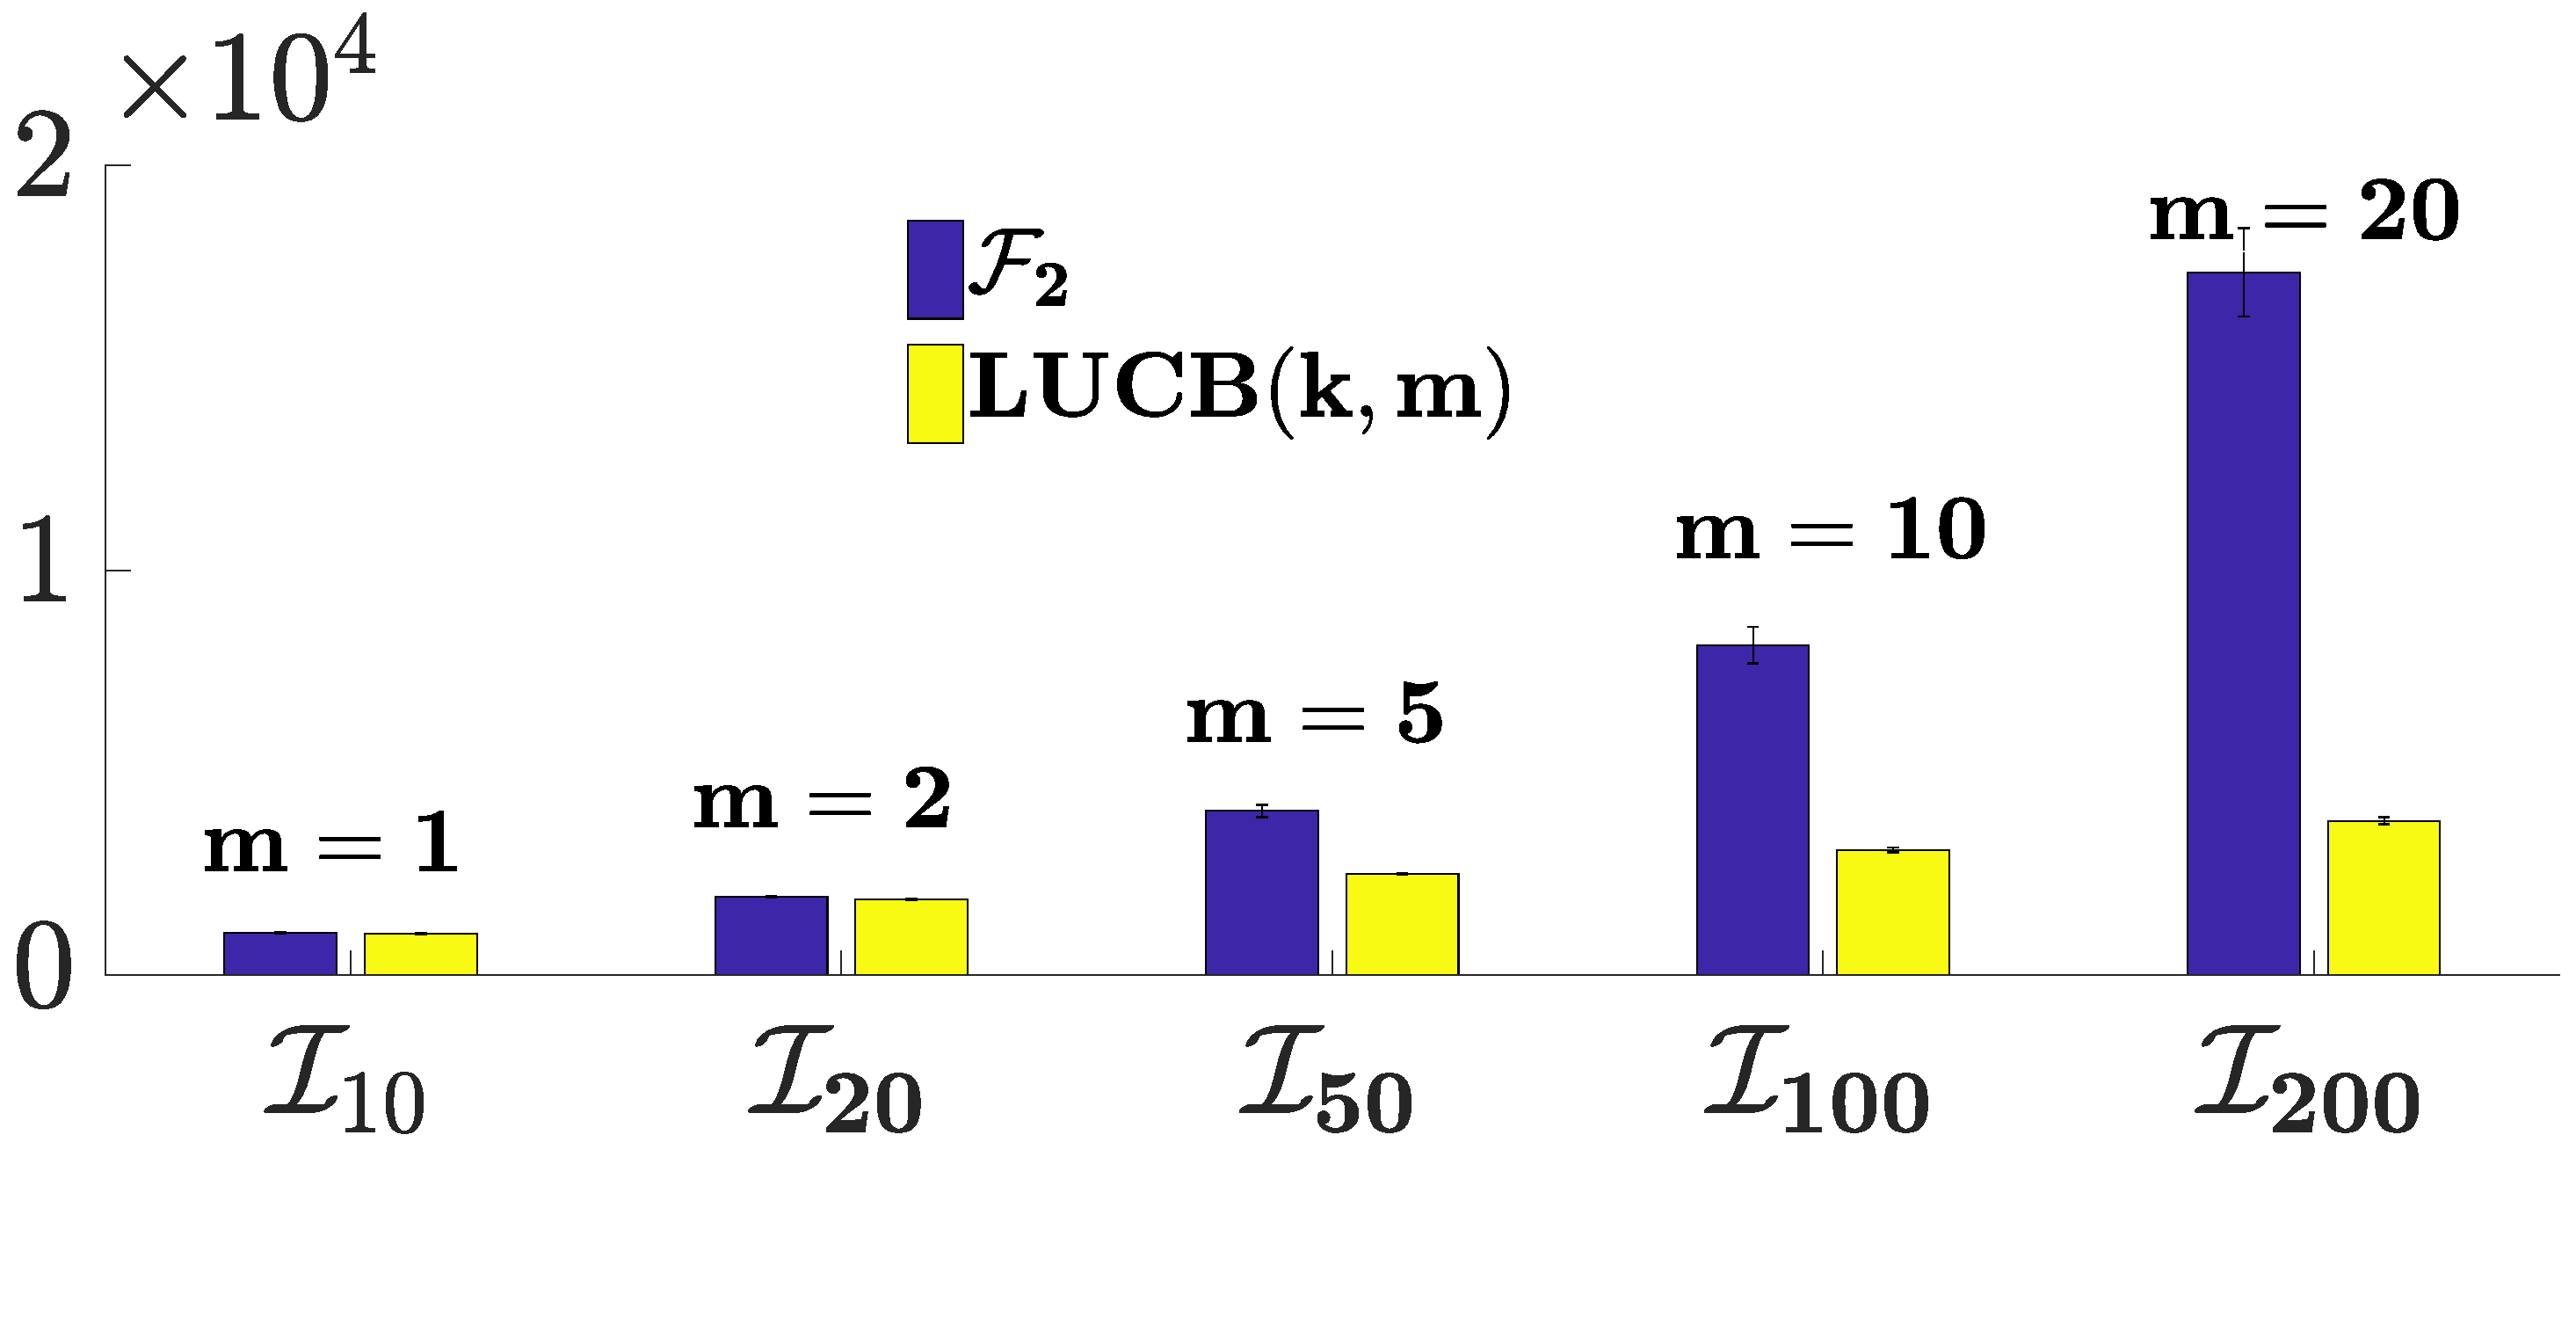
\includegraphics[width=0.35\textwidth]{compare_sc_f2_glucb_short.eps}}%
%     \subfigure[]{\label{fig:fracoptpull}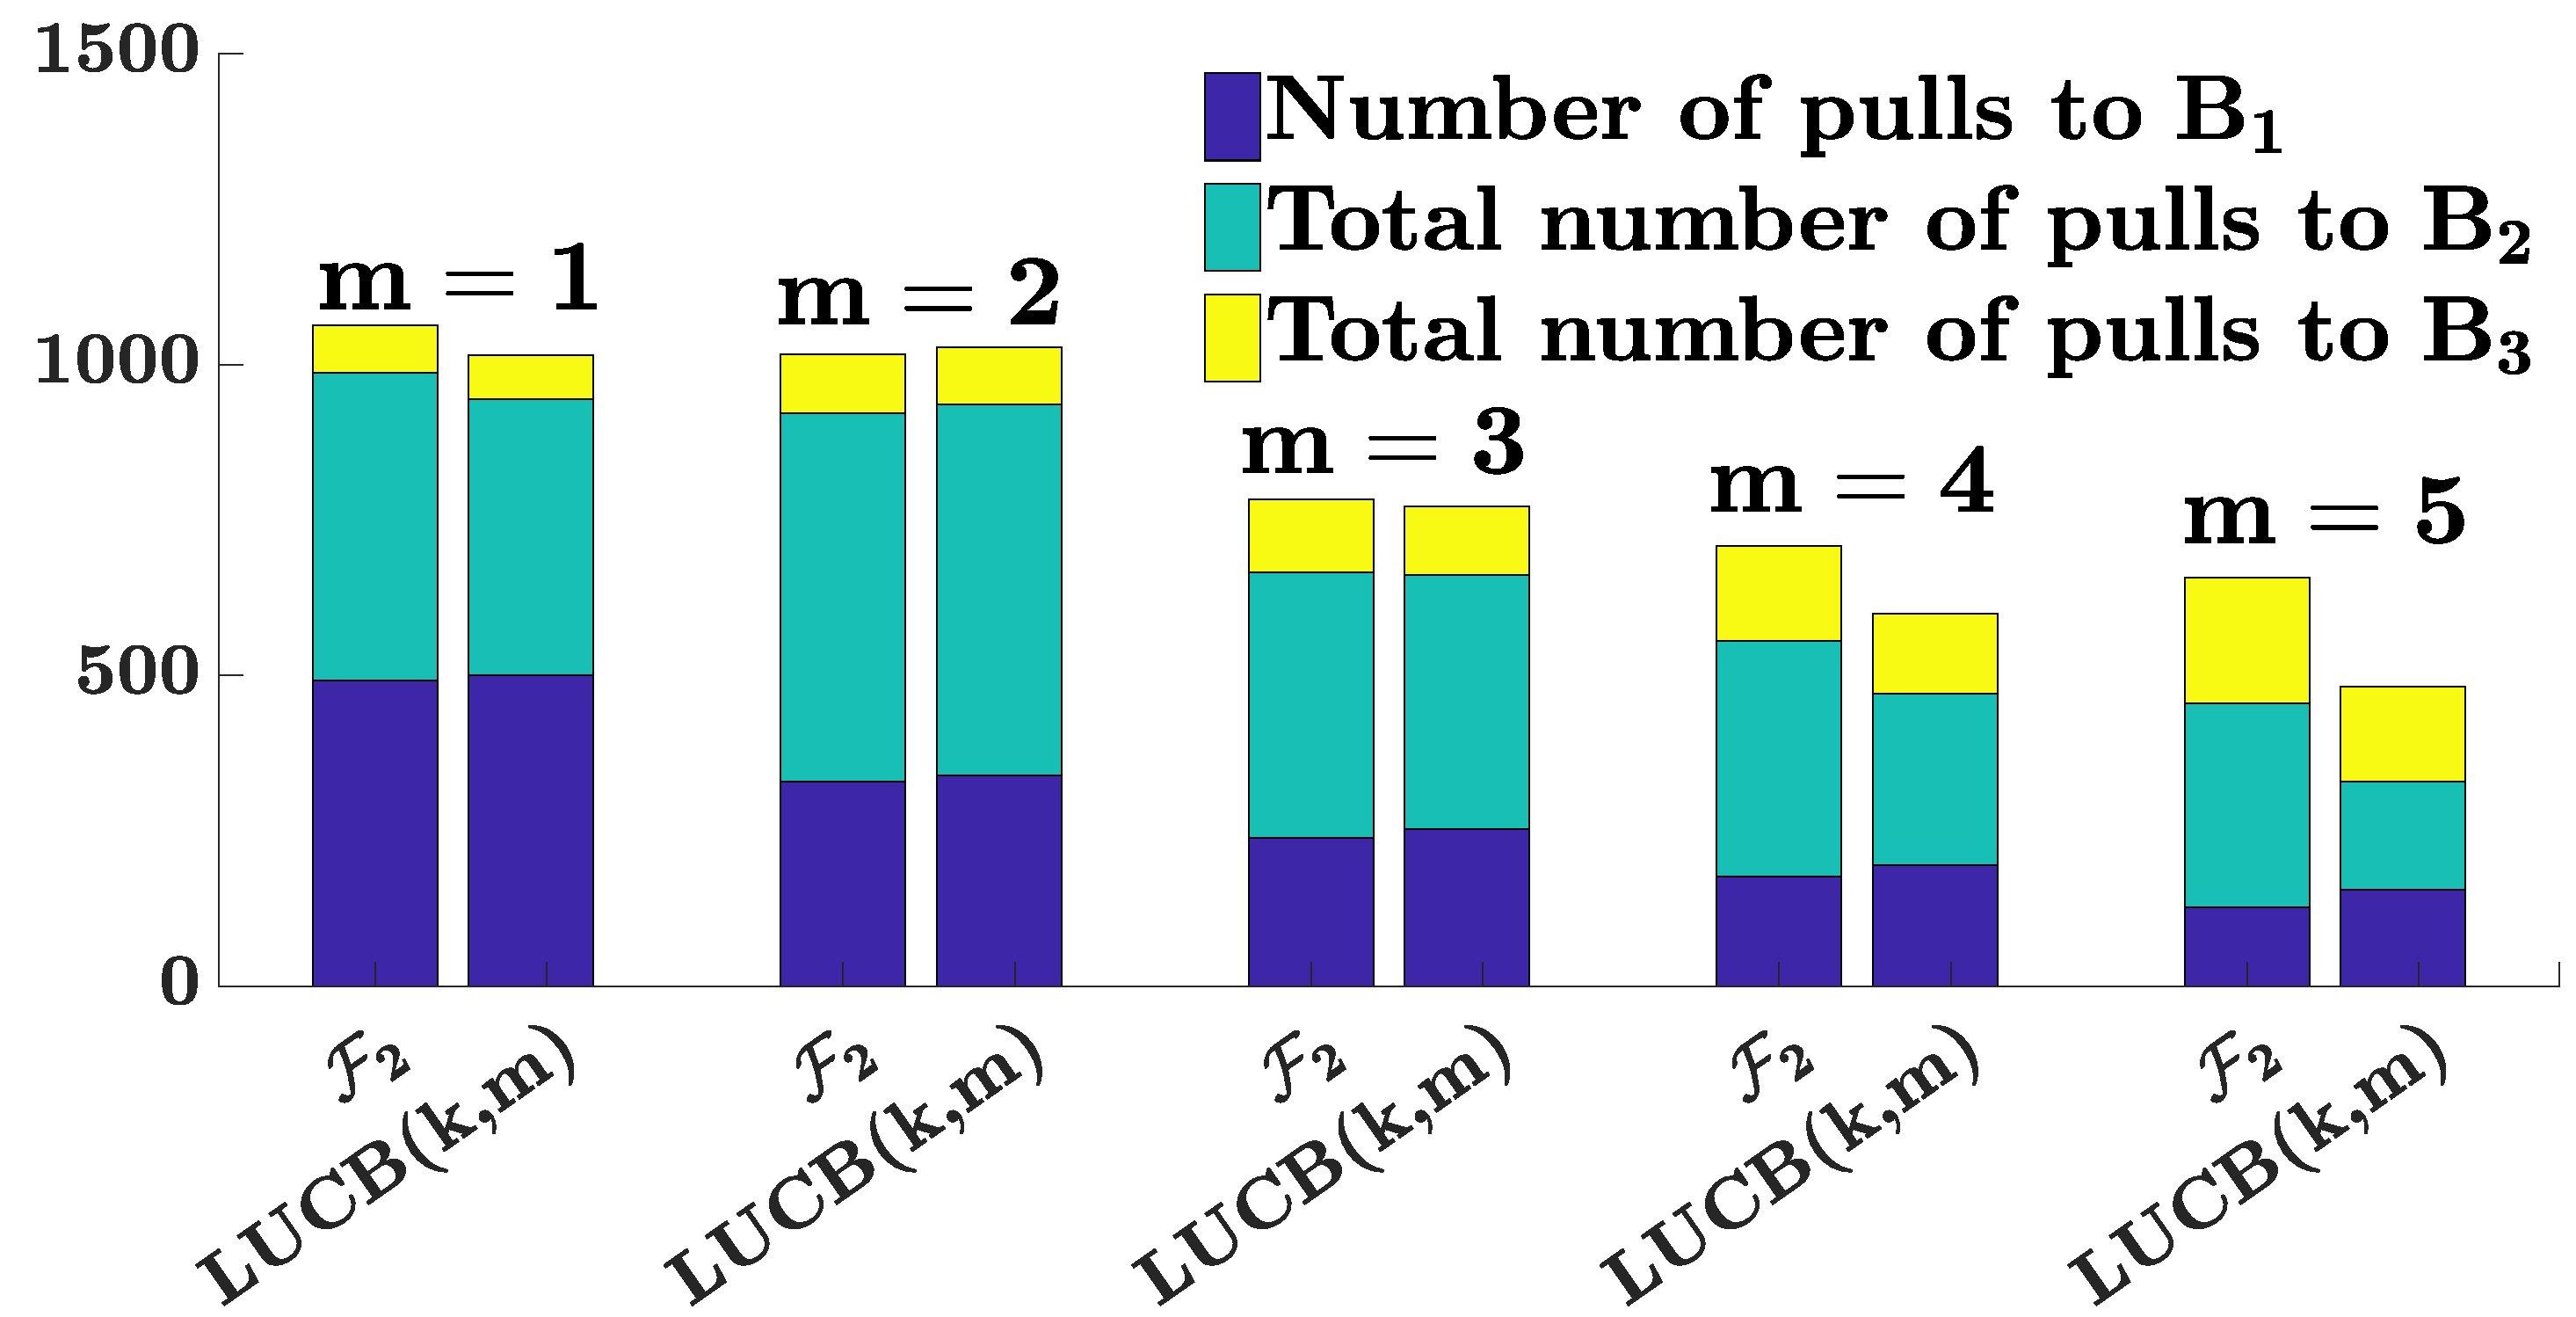
\includegraphics[height=0.95in,width=0.35\textwidth]{frac_opt_pull_short.eps}}
%     \subfigure[]{\label{fig:vark_fixtopm}\includegraphics[height=0.77in,width=0.2\textwidth]{var_k_fix_topm_short.eps}}
%  \caption{
% %  Sample complexities of \FF and \GLUCB on different instances. In all the above figures the Y-axis represents the number of samples averaged over 100 runs. Figure~\ref{fig:scf2glucb} shows a 
% %  comparison between \FF and \GLUCB on number of samples incurred to solve a \QF~\cite{bib:arcsk2017} with  $k=1$ and $m= 0.1 \times n$, on the five instances. The X-axis represents the number of arms in the corresponding instance. Figure~\ref{fig:fracoptpull} compares the number of pulls received by the camps $B_1, B_2$ and $B_3$, for solving different instances of \QF on $\I_{10}$, by varying $m$ from 1 to 5. Recall that $B_1$ is the singleton set, with the best arm being the only member. 
% % Figure~\ref{fig:vark_fixtopm} shows a comparison of the number of incurred samples by \GLUCB for solving different  instances of \QFK defined on $\I_{20}$, by setting $m = 10$, and varying $k \in \{1, 2, 3, 5, 8, 10\}$. The $\epsilon$ and $\delta$ are kept the same for all the instances and across all the experiments. For details about the instances refer Section~\ref{sec:expt}.
% In all the above figures the y-axis represents the number of samples averaged over 100 runs, with standard error bars.
% Figure~\ref{fig:scf2glucb}, and \ref{fig:fracoptpull} show comparison of sample complexities between \FF and \GLUCB.
% Figure~\ref{fig:vark_fixtopm} compares sample complexities of \QFK by keeping $m$ fixed and varying $k$.
% Details are provided in Section~\ref{sec:expt}. THERE'S ENOUGH SPACE NOW. MAKE THESE SEPARATE FIGURES AND HAVE DESCRIPTIVE CAPTIONS FOR EACH.
% }
% \label{fig:comparisons}
% \end{figure*}

As shown by \citet{Jamieson+N:2014} the efficiency of \LUCB comes from the quick identification of the most 
optimal arm due to a large separation from the $m+1$-th arm.
Intuitively, the possible reason for \FF to incur more samples is the delay in prioritising the 
optimal arm to pull more frequently. This should result in a smaller fraction of total samples taken from the best 
arm. Figure~\ref{fig:fracoptpull} affirms this intuition. It represents a comparison between \FF and \GLUCB on the number of samples obtained by
three ``ground-truth'' groups---$B_1$, $B_2$, and $B_3$
on $\I_{10}$, keeping $k=1$ and varying $m$ from 1 to 5. We note that
the lesser the difference between $k$ and $m$, the higher the hardness ($H_\epsilon$), and
both \FF and \GLUCB find it hard to identify a correct arm. Hence, for $k = m =1$, both of them
spend almost the same fraction of pulls to the best arm.
However, as $m$ becomes larger, keeping $k=1$, the hardness of the problem reduces, but
\FF still struggles to identify the best arm and results in spending a significantly
a lesser fraction of the total pulls to it, compared to \GLUCB. 

In this paper, we have developed algorithms specifically for the \QFK problem; previously one might have solved \QFK either by solving $(k, k, n)$ or $(m, m, n)$: that is choosing the \textit{best} $k$- or $m$-sized subset.  In Figure~\ref{fig:vark_fixtopm} we present a comparison of the sample complexities 
for solving  \QFK and the best subset-selection problems. 
Fixing $\A = \I_{20}$, $n=20$, $m = 10$, \QFK instances 
are given by and varying $k \in \{1, 3, 5, 8, 10\}$, whereas, for the best subset-selection problem we set $m =k$.
As expected, the number of samples incurred is significantly lesser for solving the problem instances with $k < m$, thereby validating the use of \GLUCB. %\filler{Best to place figures and tables Top or Bottom rather than Here.}

% Recalling the fact that for $k = m$, \GLUCB exactly coincides with \LUCB,  in Figure~\ref{fig:vark_fixtopm}
% we present a comparison of their complexities
% on $\I_{20}$, fixing $m = 10$, and varying $k \in \{1, 3, 5, 8, 10\}$. As expected, the number of samples 
% incurred by \GLUCB for solving \QFK with $k < m$, is far below that for solving $k = m$.

% We study how does the number of samples by \GLUCB increases with $k$. Considering $\I_{20}$, fixing $m = 10$, 
% for $k \in \{1, 3, 5, 8, 10\}$,
% we plot the number of samples incurred by \GLUCB in Figure~\ref{fig:vark_fixtopm}.

% {\color{blue} By definition, \GLUCB exactly coincides with LUCB for $k == m$.).}

% We notice that for $k = 1, 2, 3, 5, 8$, and $10$, $H_\epsilon = 396.4, 1029.7, 1428.6,
% 2225.9, 3420.3$, and $4214.8$ respectively. Therefore, 
% as supported by the theory, the number of 
% samples drawn by \GLUCB increases rapidly as $k$ gets closer to $m$.


\begin{figure}[h]
\centering
 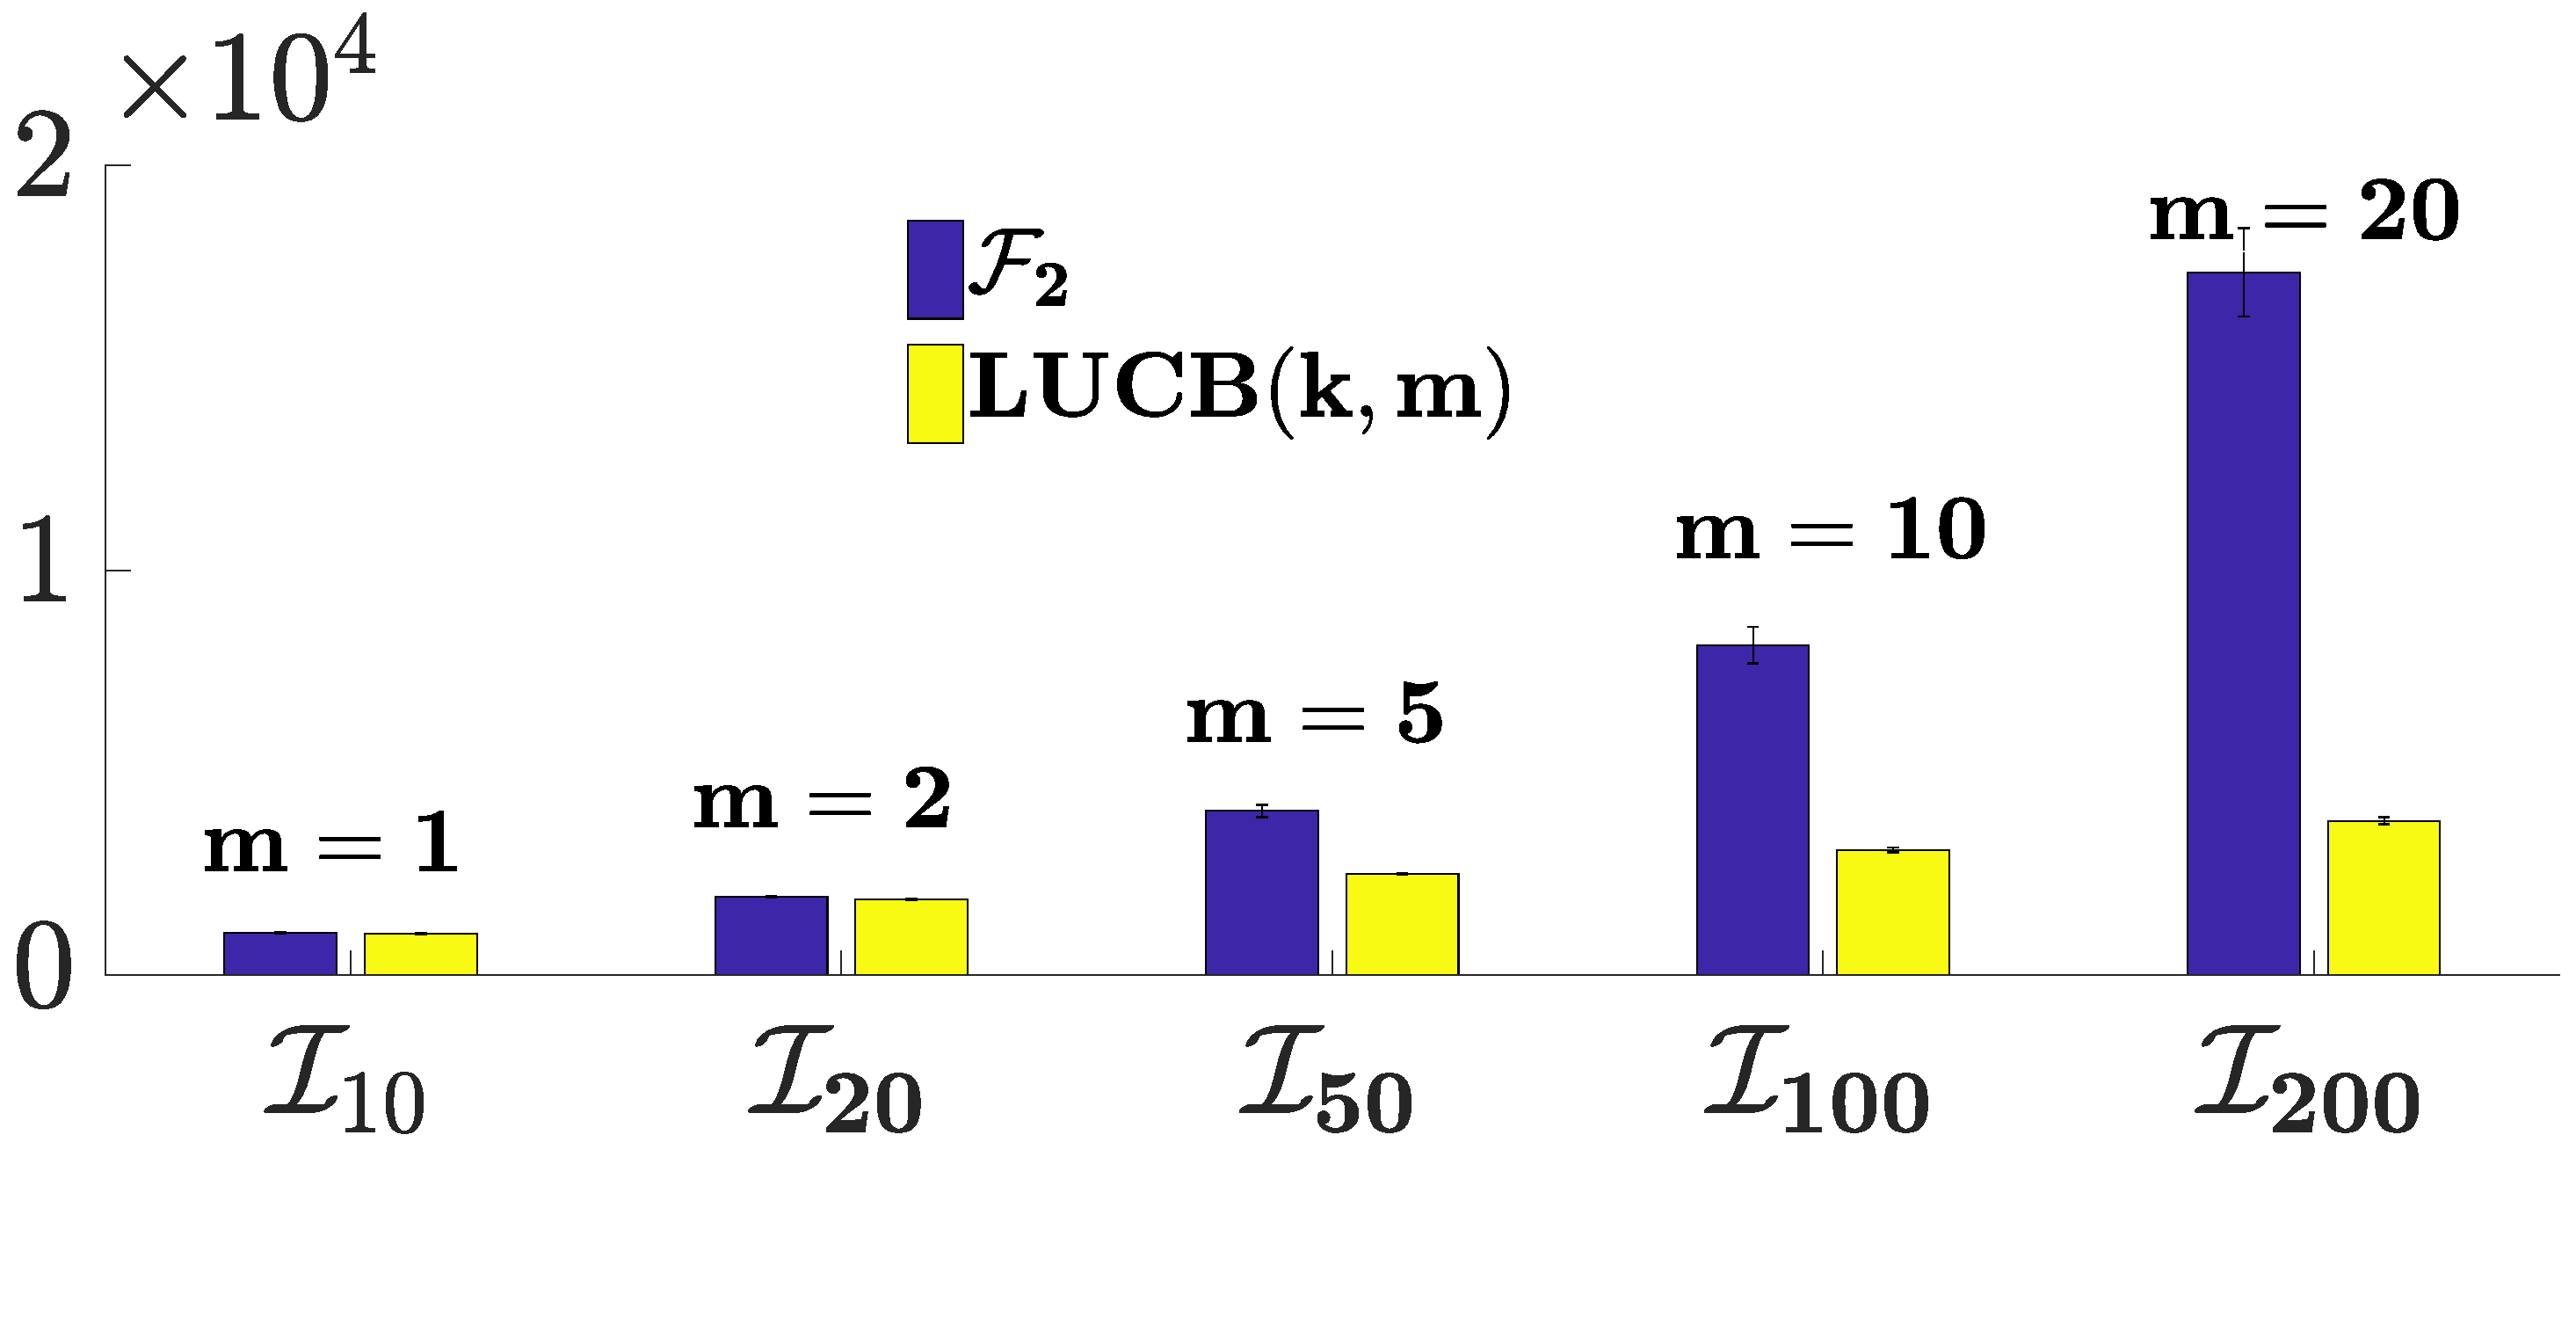
\includegraphics[height=1.2in]{compare_sc_f2_glucb_short.eps}
 \caption{Comparison of incurred sample complexities by \FF and \GLUCB 
	  to solve \QF with  $m= 0.1 \times n$, on the five instances
	  detailed in Section~\ref{sec:expt}.
	  y-axis represents the number of samples averaged over 100 runs, with standard error bars.}
 \label{fig:scf2glucb}
\end{figure}

\begin{figure}[h]
\centering
 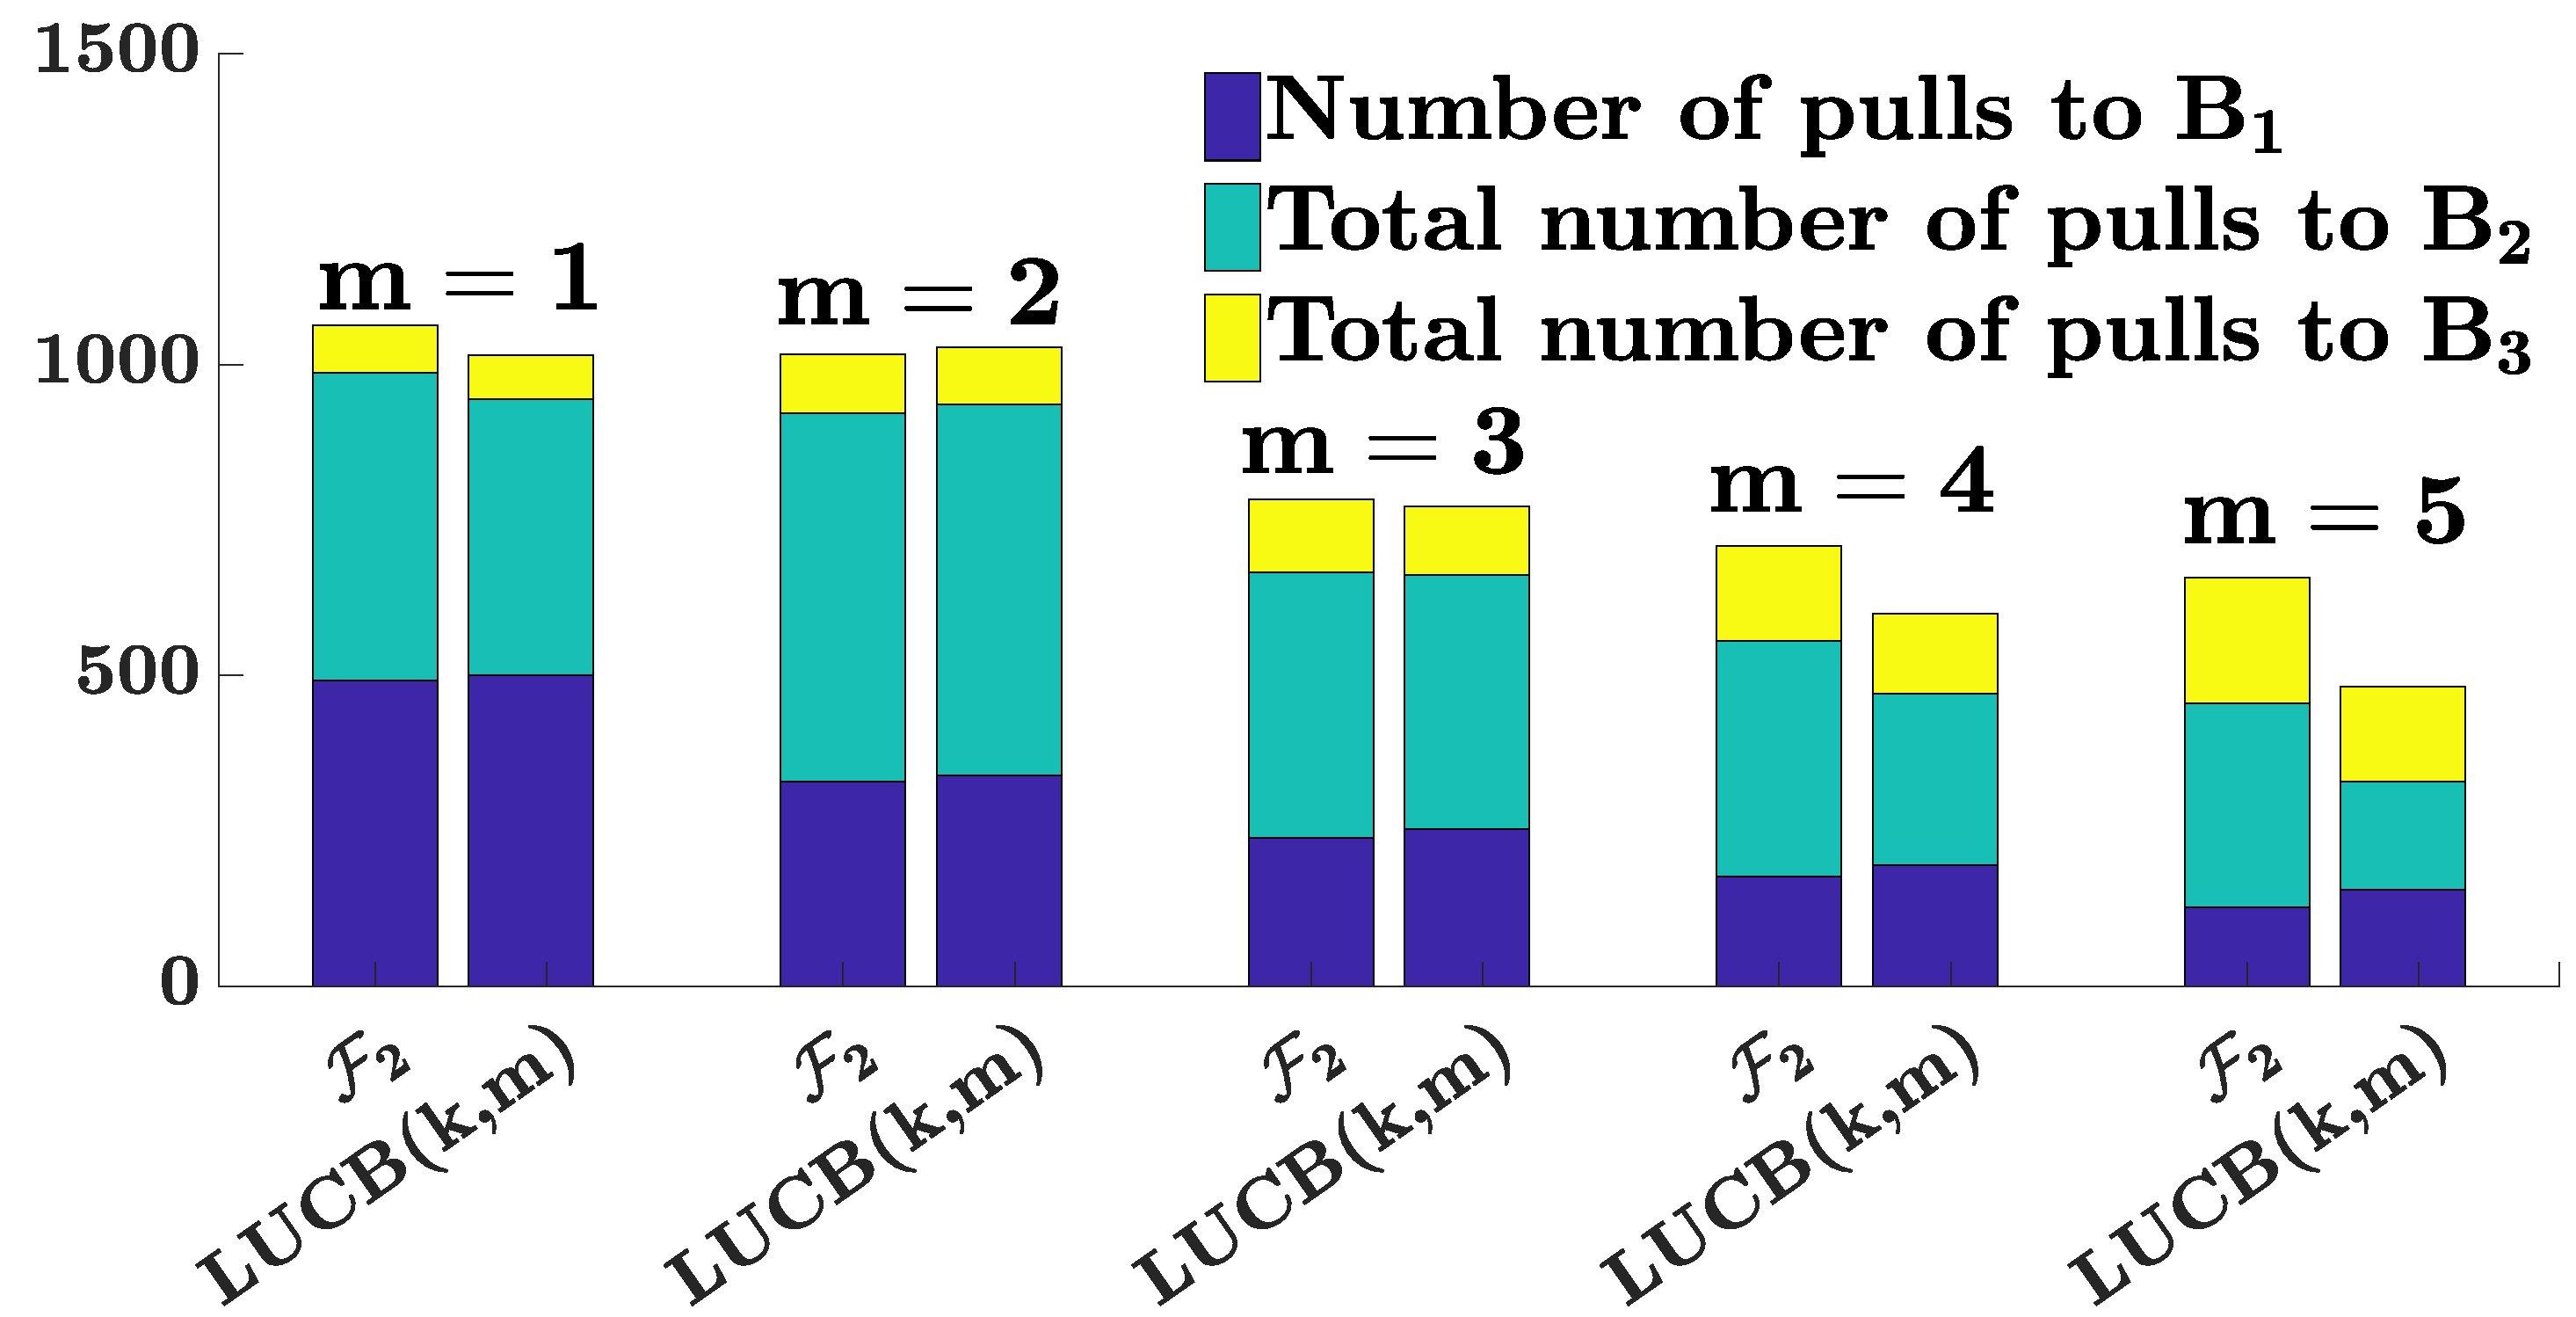
\includegraphics[height=1.5in]{frac_opt_pull_short.eps}
 \caption{Comparison between \FF and \GLUCB on the number of
	  pulls received by the camps $B_1, B_2$ and $B_3$, for solving
	  different instances of \QF on $\I_{10}$, by varying $m$ from 1 to 5. 
	  Recall that $B_1$ is the singleton set, with the best arm being 
	  the only member. y-axis represents the number of samples averaged over 100 runs.}
 \label{fig:fracoptpull}
\end{figure}

\begin{figure}[h]
\centering
 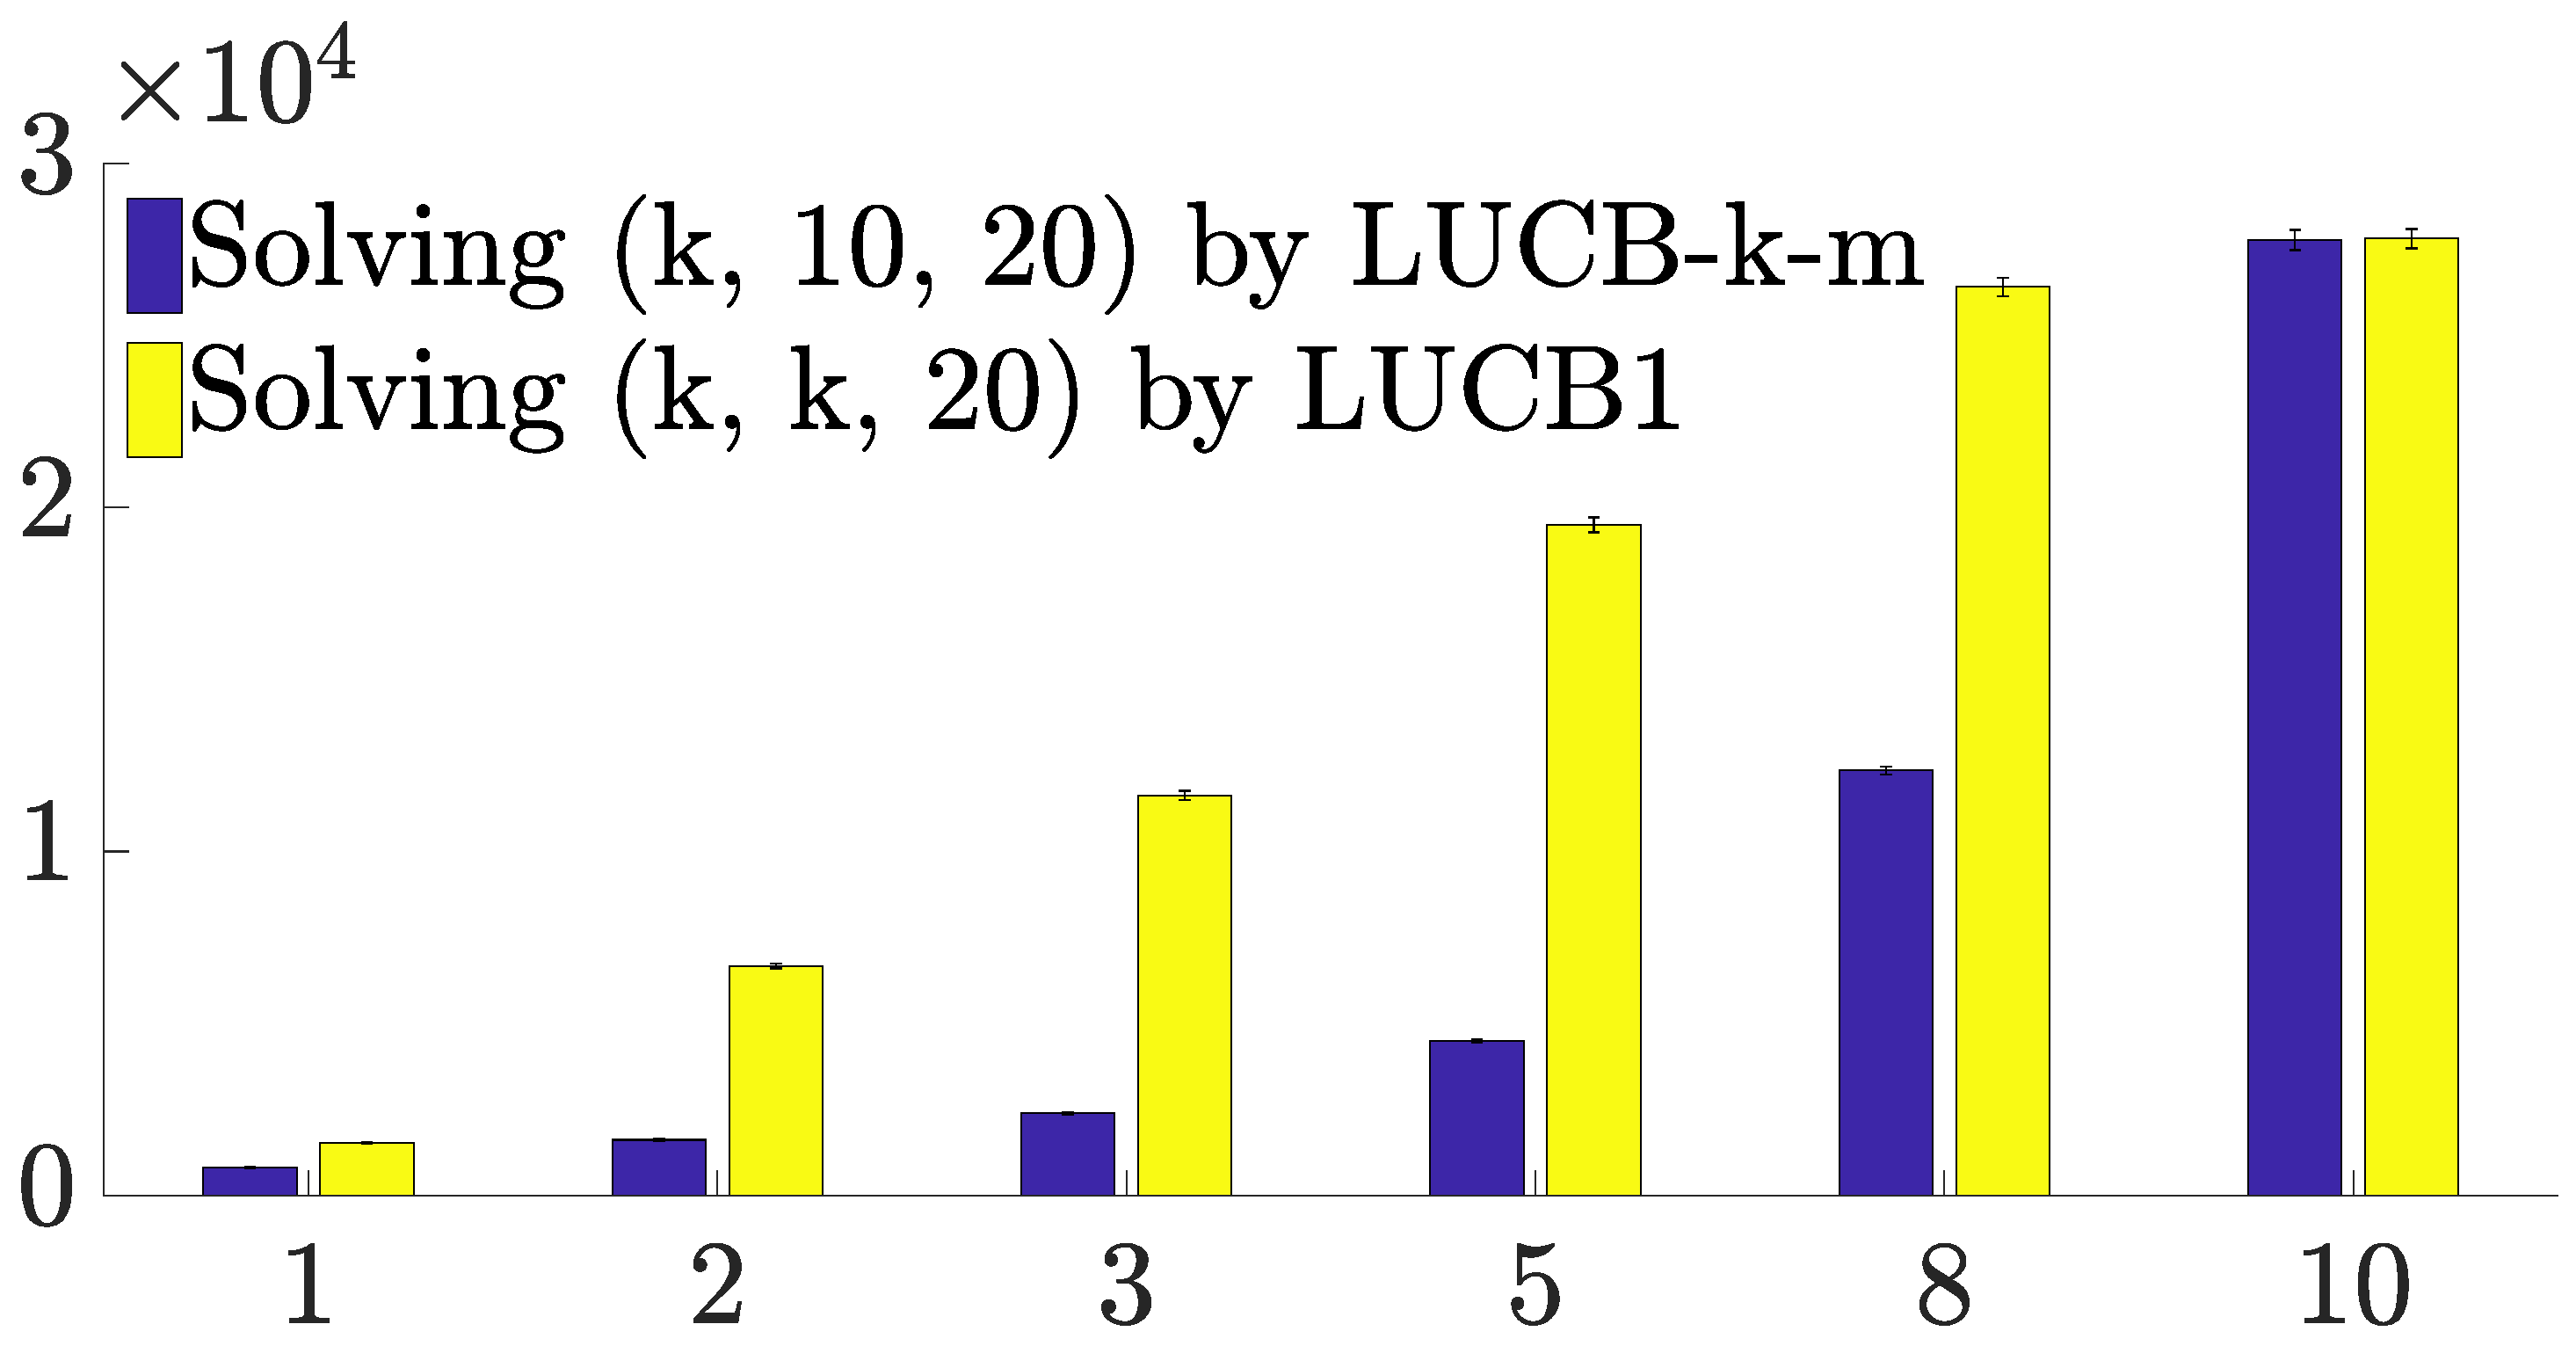
\includegraphics[height=1.2in]{comp_glucb_var_k.eps}
 \caption{ Comparison of number of samples incurred for 
%  Comparison of sample complexities of incurred samples by \GLUCB for 
	  solving different  instances of \QFK defined on $\I_{20}$, by 
	  setting $m = 10$, and varying $k \in \{1, 2, 3, 5, 8, 10\}$.
	  x-axis represents $k$, and y-axis represents the number of samples 
	  averaged over 100 runs, with standard error bars.}
 \label{fig:vark_fixtopm}
\end{figure}
